\documentclass[aspectratio=169, 10pt]{beamer}

% Packages
\usepackage[utf8]{inputenc}
\usepackage{graphicx}
\usepackage{booktabs}
\usepackage{amsmath}
\usepackage{xcolor}
\usepackage{tikz}

% Theme
\usetheme{Madrid}
\usecolortheme{default}
\setbeamertemplate{navigation symbols}{}

% Title Information
\title[Fact Omission vs. Rhetorical Framing]{Fact Omission vs. Rhetorical Framing: \\ Disentangling the Predictors of Media Bias}
\author[Sai, Batra, More]{Aditya Sai, Aayush Batra, Yash More}
\institute[IIIT Hyderabad]{IIIT Hyderabad}
\date{April 2026}

\begin{document}

% Slide 1: Title
\begin{frame}
    \titlepage
\end{frame}

% Slide 2: Motivation & Problem Statement
\begin{frame}{Motivation \& Problem Statement}
    \textbf{How do we detect Media Bias?}
    \vspace{0.3cm}
    \begin{itemize}
        \item Traditional bias detection focuses heavily on \textbf{lexical choices} (word choice, sentiment, framing language).
        \item However, bias also manifests through \textbf{structural choices}:
        \begin{itemize}
            \item Which facts to include or omit? (Selection Bias)
            \item Where to position facts within the discourse? (Framing Bias)
        \end{itemize}
    \end{itemize}
    
    \vspace{0.4cm}
    \begin{block}{Our Core Question}
    Is media bias better predicted by \textbf{fact omission} (what is not said) or by the \textbf{rhetorical positioning} of shared facts (how it is structured)?
    \end{block}
\end{frame}

% Slide 3: Two-Tier Hypothesis
\begin{frame}{The Two-Tier Hypothesis of Media Bias}
    We hypothesized that media bias operates on two structural tiers:
    \vspace{0.5cm}
    
    \begin{columns}
        \column{0.48\textwidth}
        \begin{block}{Tier 1: Selection Bias (Omission)}
        Sources choose \textit{which} facts to report, creating coverage asymmetries.
        \begin{itemize}
            \item A left-leaning source might omit a fact that a right-leaning source emphasizes.
        \end{itemize}
        \end{block}
        
        \column{0.48\textwidth}
        \begin{block}{Tier 2: Framing Bias (RST Structure)}
        For facts that are shared, the rhetorical positioning differs.
        \begin{itemize}
            \item We use \textbf{Rhetorical Structure Theory (RST)} to quantify if a fact is the "nucleus" (core message) or a "satellite" (background).
        \end{itemize}
        \end{block}
    \end{columns}
\end{frame}

% Slide 4: Dataset & Triplets
\begin{frame}{Dataset \& Triplet Construction}
    \begin{itemize}
        \item \textbf{Source:} 37,554 labeled news articles from AllSides.com.
        \item \textbf{Triplets:} We grouped articles covering the \textit{exact same event} into triplets: (1 Left, 1 Center, 1 Right).
        \item \textbf{RST Parsing:} We processed articles to build discourse trees consisting of Elementary Discourse Units (EDUs, i.e., facts/clauses).
    \end{itemize}
    
    \vspace{0.4cm}
    \textbf{Final Usable Dataset:}
    \begin{itemize}
        \item \textbf{1,748 Valid Triplets} (split securely into 80/10/10 Train/Val/Test with no article leakage).
        \item \textbf{548,960 high-quality EDUs}.
    \end{itemize}
\end{frame}

% Slide 5: The Bipartite Approach (Methodology)
\begin{frame}{The Bipartite Matching Approach}
    \textbf{How do we compare structures across three different articles?}
    \vspace{0.3cm}
    \begin{itemize}
        \item We first \textbf{cluster similar facts} across the triplet using SBERT embeddings and a Cross-Encoder.
        \item Then we apply our novel \textbf{Bipartite Approach}:
        \begin{enumerate}
            \item We perform 1-to-1-to-1 matching to align EDUs (Left vs Center, Right vs Center).
            \item We generate \textbf{Structural Features}: Difference in rhetorical depth/prominence between matched facts.
            \item We generate \textbf{Coverage Features}: Explicit flags (+1 / -1 / 0) for when one side has a fact but the other omits it.
        \end{enumerate}
    \end{itemize}
    \vspace{0.2cm}
    \textit{This approach explicitly encodes both the framing and the omission signals into the Discourse Framing Index (DFI) vector.}
\end{frame}

% Slide 6: Results - Full Classification
\begin{frame}{Classification Results: Full Dataset}
    \textbf{Task:} Given a document's DFI vector compared to the Center, predict if it is Left or Right.
    \vspace{0.3cm}
    
    \begin{table}[]
        \centering
        \large
        \begin{tabular}{lc}
        \toprule
        \textbf{Method} & \textbf{Test Accuracy} \\
        \midrule
        \textbf{Bipartite Coverage + RF} & \textbf{89.77\%} \\
        Bipartite Combined + RF & 88.07\% \\
        Padded DFI + RF & 87.78\% \\
        Padded DFI + SVM & 85.23\% \\
        \bottomrule
        \end{tabular}
    \end{table}
    
    \vspace{0.3cm}
    \begin{itemize}
        \item \textbf{Random Forest (RF)} significantly outperformed SVMs because it inherently handles categorical coverage deltas ($\{-1, 0, +1\}$) and padded arrays better.
    \end{itemize}
\end{frame}

% Slide 7: The Discovery - Shared Facts Drop-Off
\begin{frame}{The Discovery: How Many Facts Are Actually Shared?}
    When we analyzed the clusters, we found a stark reality about modern media: \textbf{left and right sources rarely report the exact same facts.}
    
    \vspace{0.3cm}
    \begin{columns}
        \column{0.5\textwidth}
        \begin{figure}
            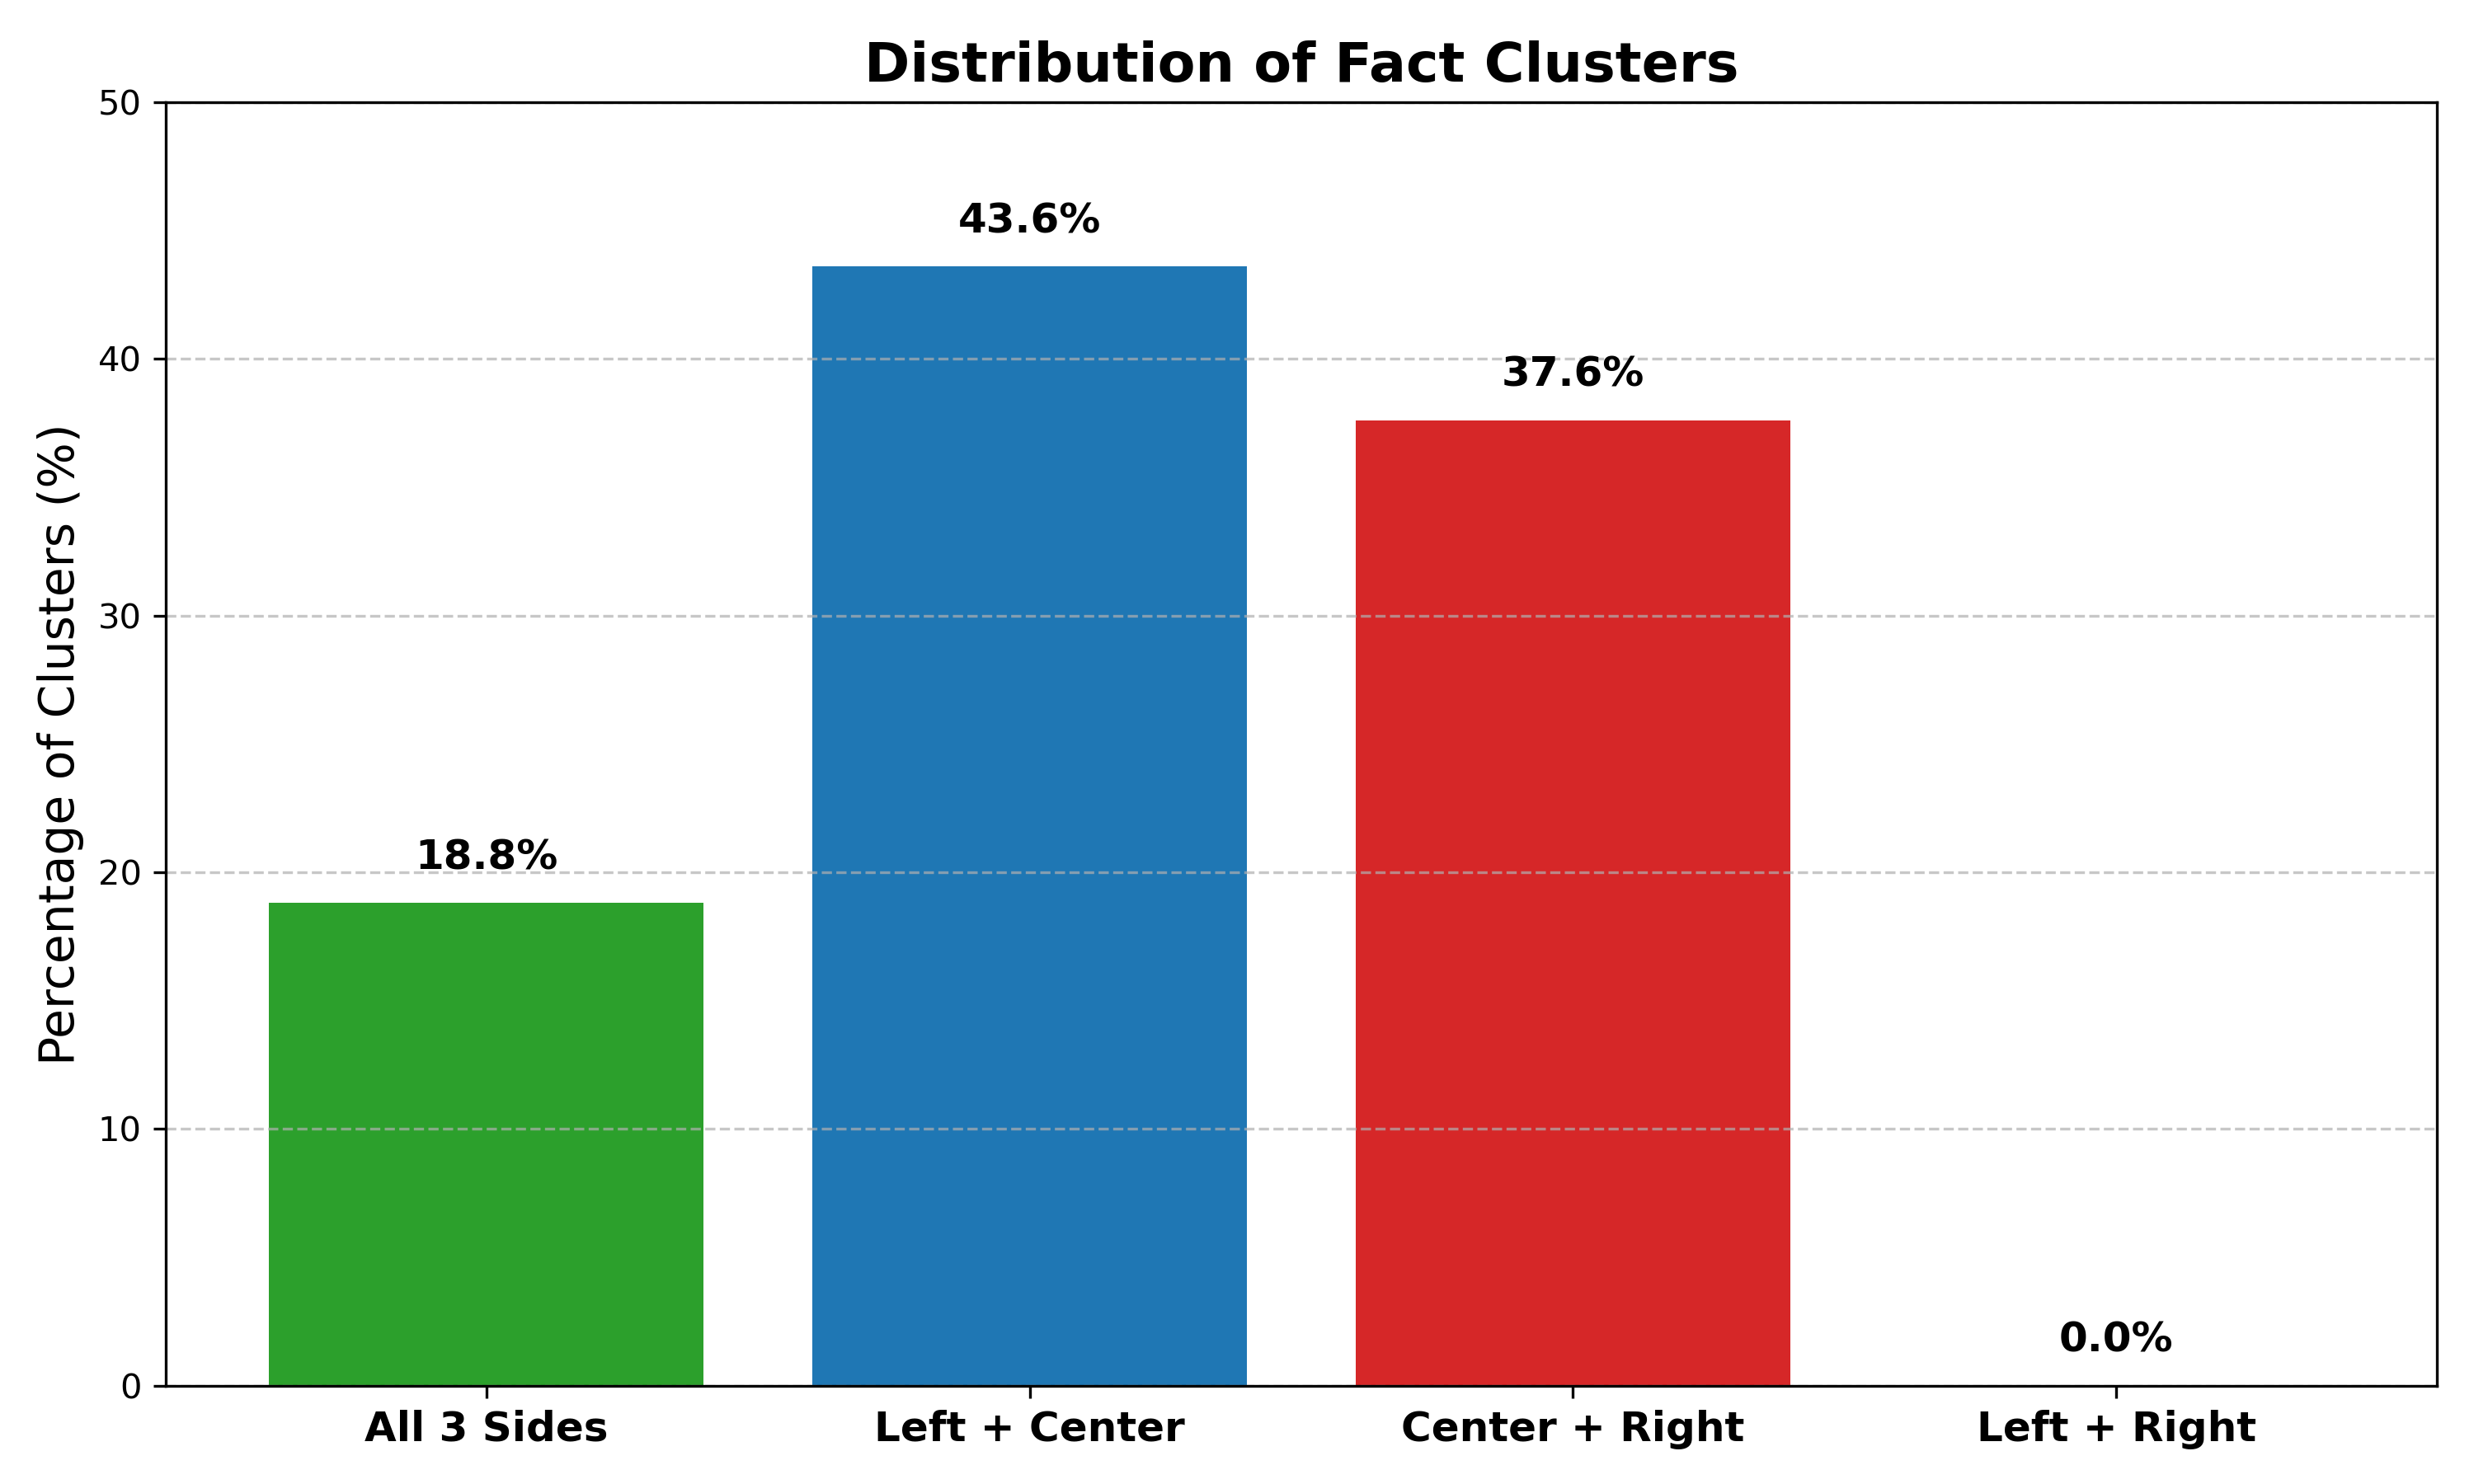
\includegraphics[width=\textwidth]{diagrams/cluster_distribution.png}
        \end{figure}
        
        \column{0.5\textwidth}
        \begin{itemize}
            \item Only \textbf{18.8\%} of fact clusters exist in all three sources.
            \item On average, a triplet shares only \textbf{3.95 facts} across the entire event.
            \item \textbf{24.4\% of triplets (427)} have \textit{zero} 3-way shared facts.
        \end{itemize}
    \end{columns}
\end{frame}

% Slide 8: The 3-Way Experiment (Isolating Framing)
\begin{frame}{The 3-Way Experiment: Isolating Framing Bias}
    What happens if we \textit{remove} the omission signal entirely? We evaluated the model exclusively on facts reported by \textbf{all three sides}.
    
    \vspace{0.3cm}
    \begin{columns}
        \column{0.5\textwidth}
        \begin{figure}
            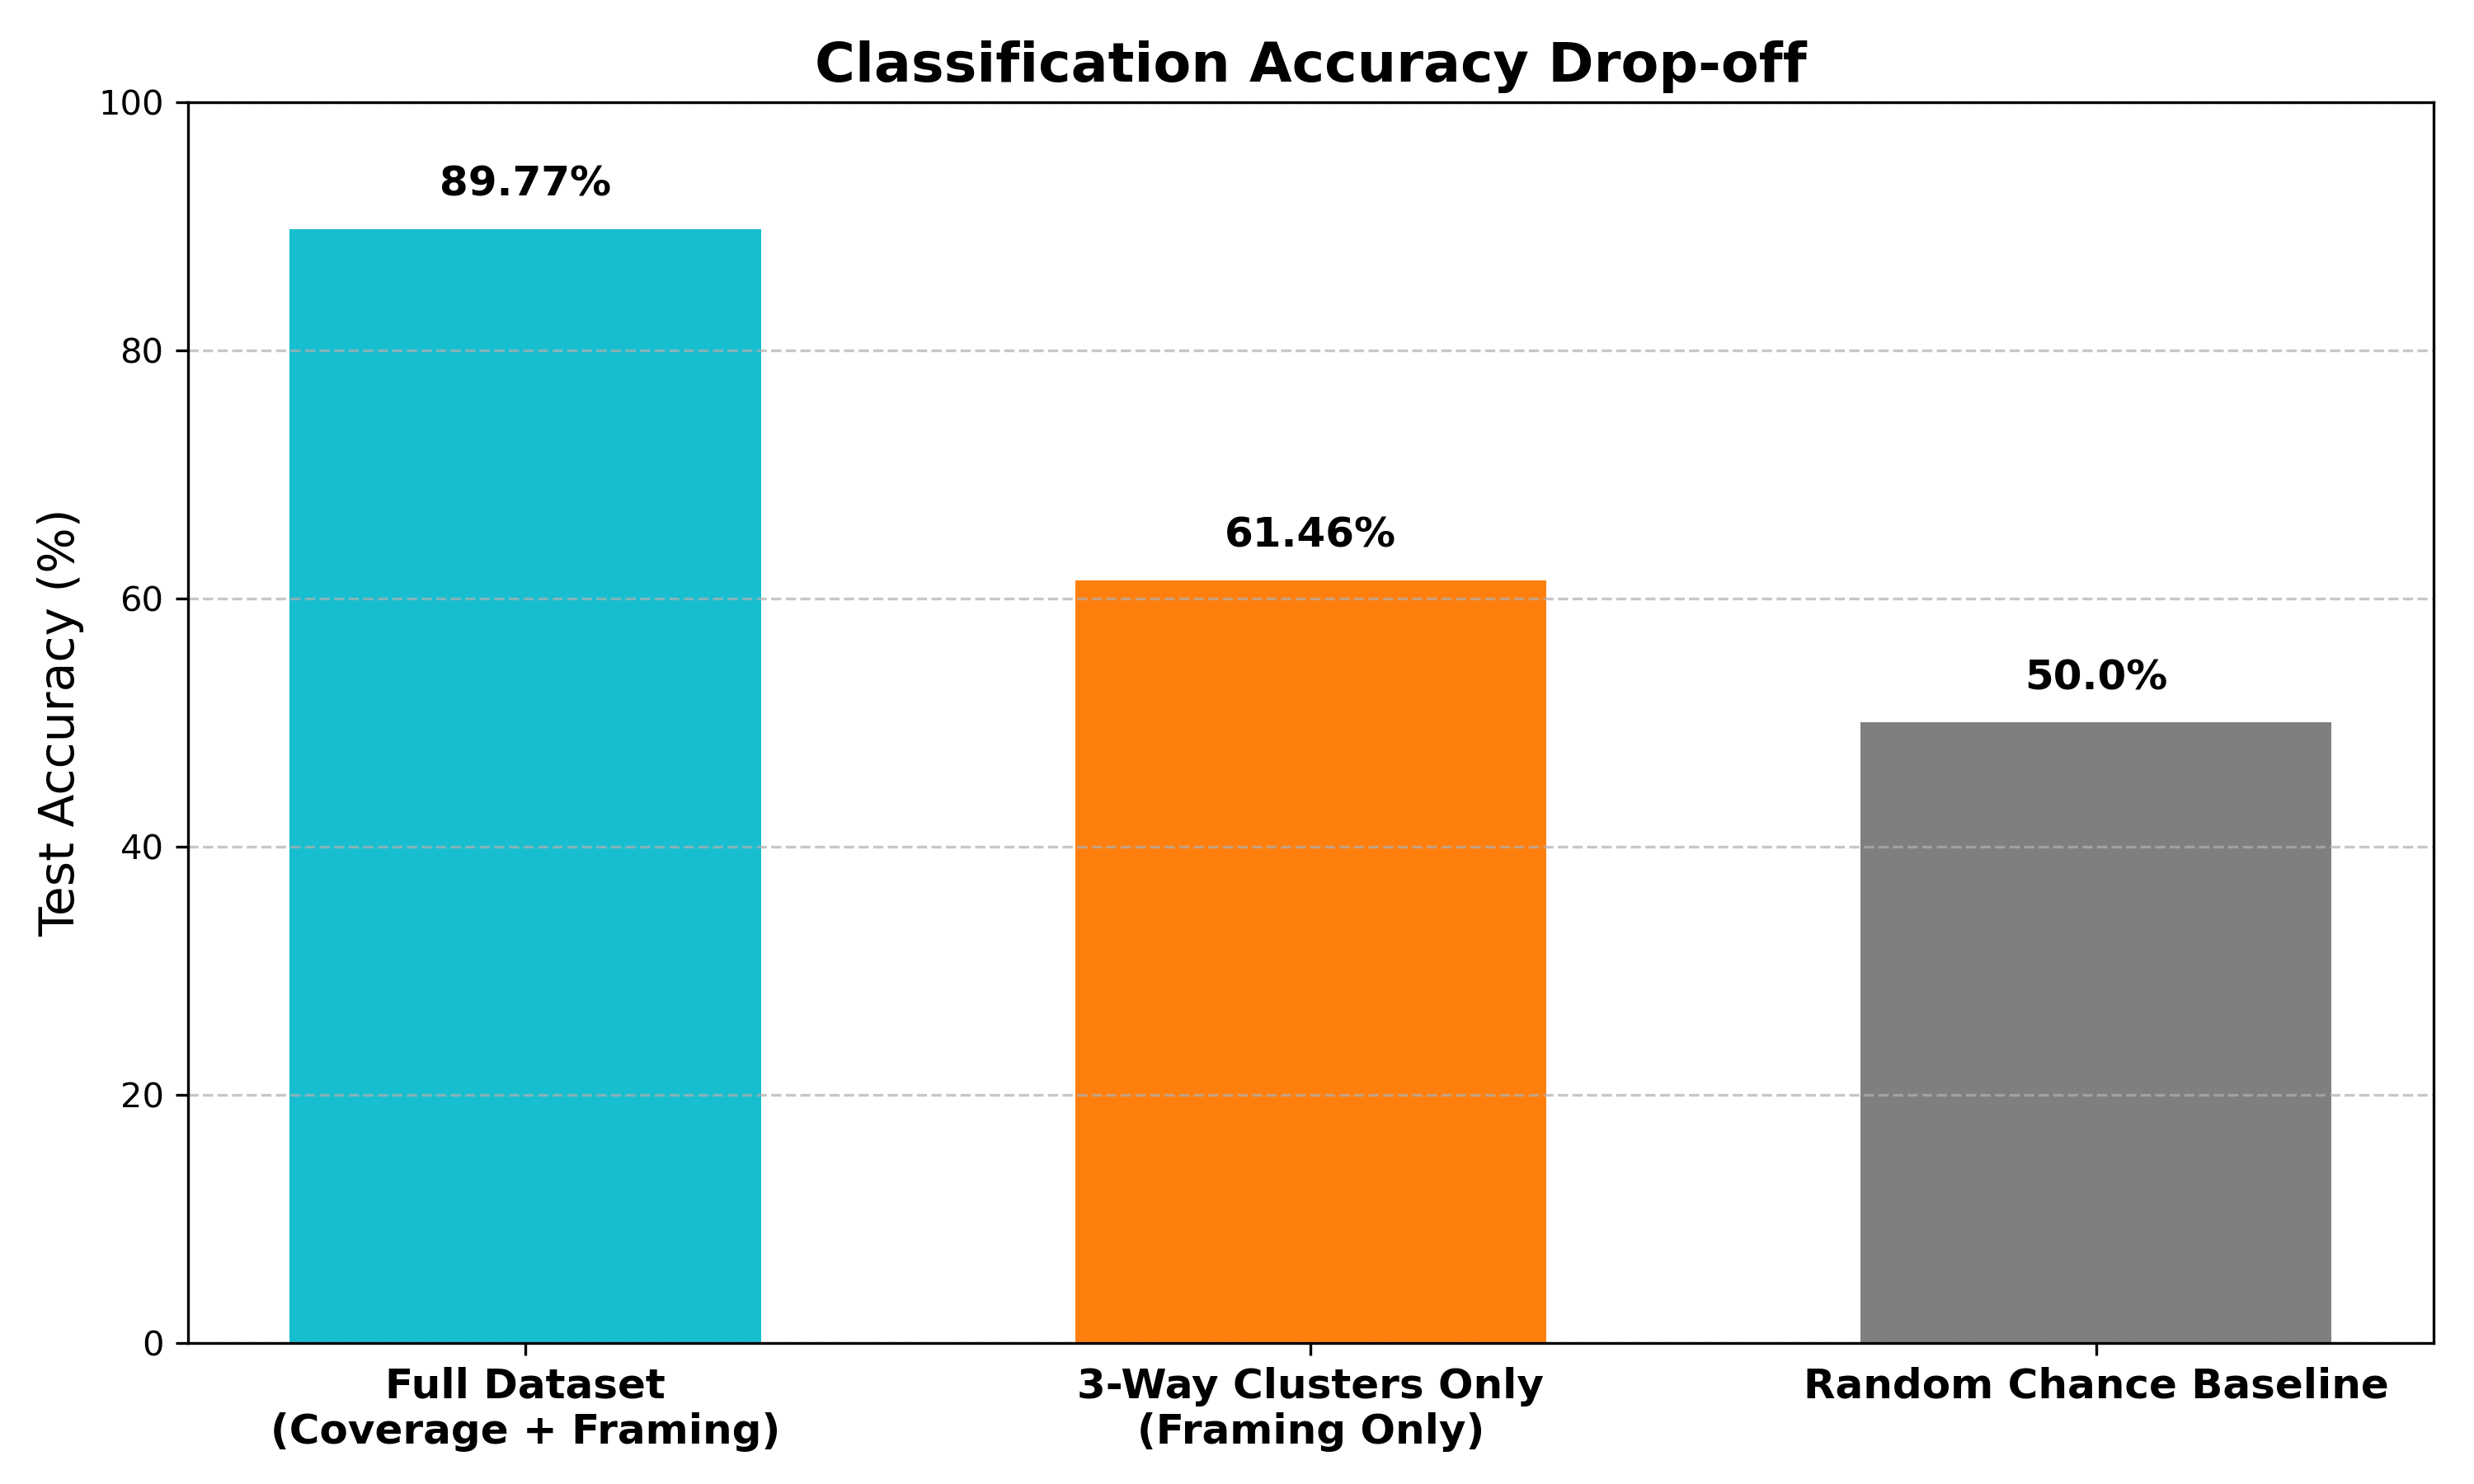
\includegraphics[width=\textwidth]{diagrams/performance_drop.png}
        \end{figure}
        
        \column{0.5\textwidth}
        \begin{itemize}
            \item With omission removed, accuracy plummeted from \textbf{89.77\%} to \textbf{61.46\%}.
            \item This is barely above the \textbf{50\% random chance baseline}.
            \item Conclusion: Framing alone is a weak predictor of bias compared to omission.
        \end{itemize}
    \end{columns}
\end{frame}

% Slide 9: Quantifying the Contributions
\begin{frame}{Predictive Power: Omission vs. Framing}
    By comparing the performance drops, we quantified the relative contribution of each tier:
    
    \vspace{0.3cm}
    \begin{columns}
        \column{0.5\textwidth}
        \begin{figure}
            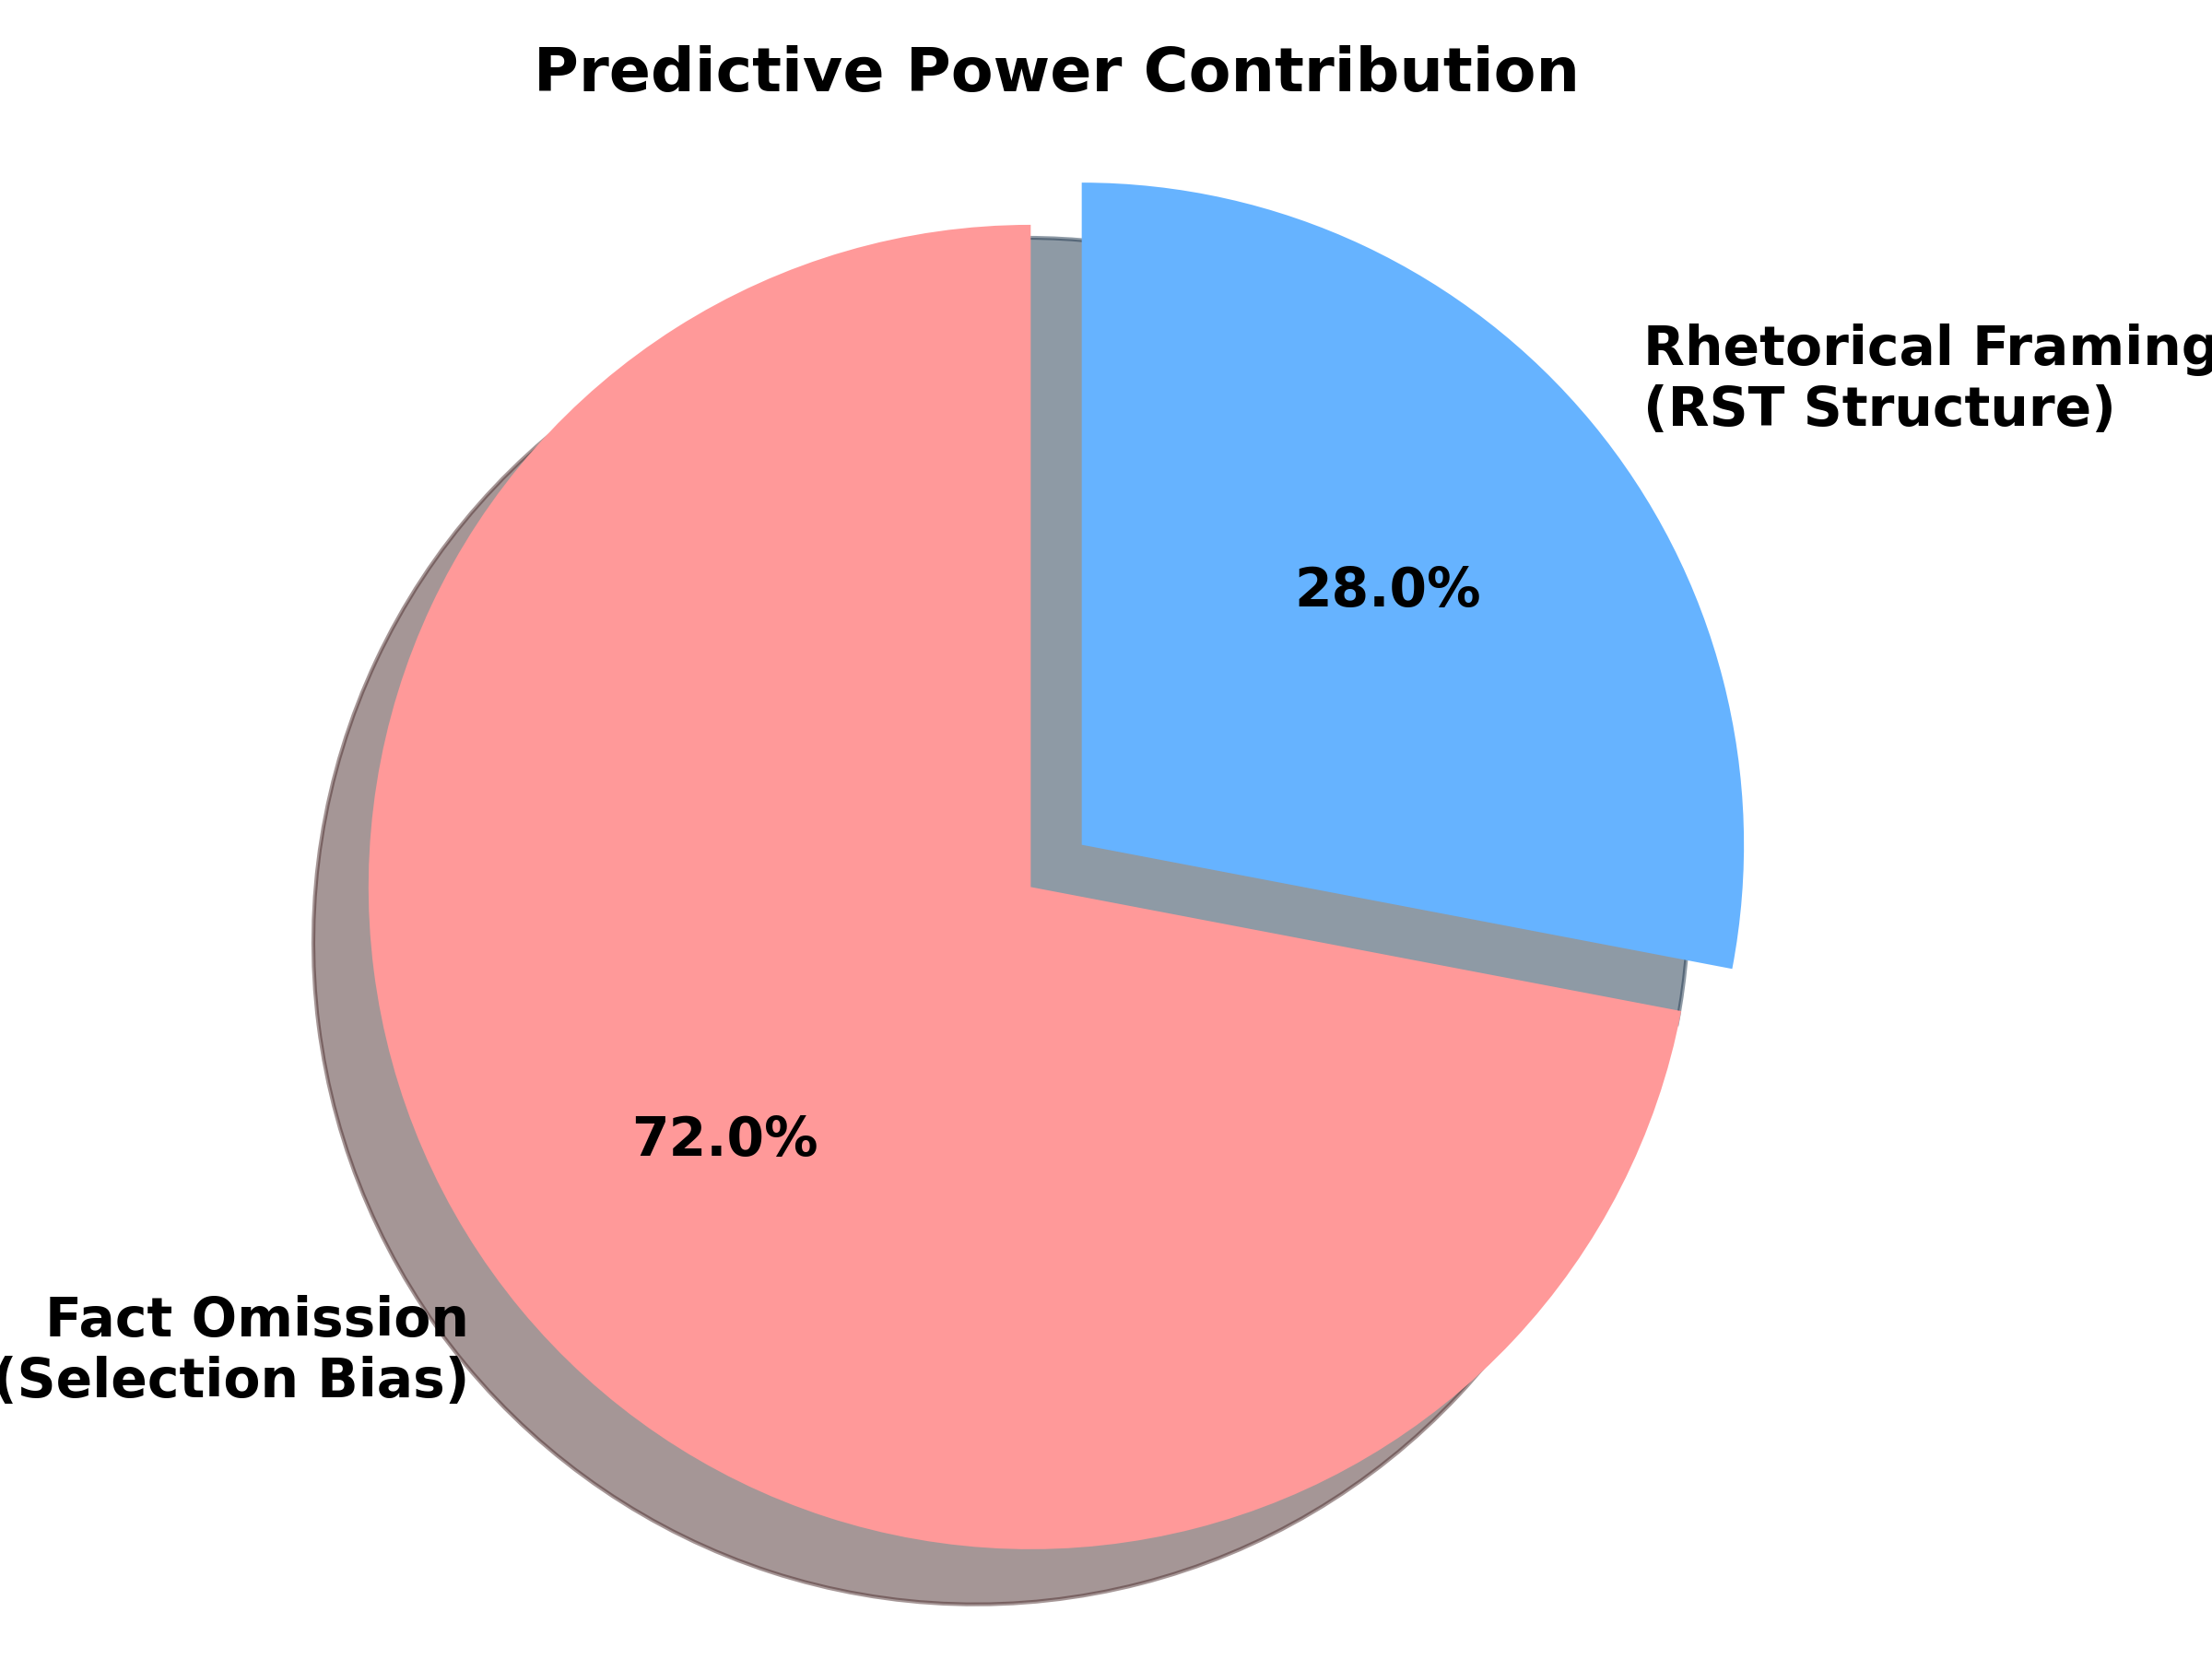
\includegraphics[width=\textwidth]{diagrams/omission_vs_framing.png}
        \end{figure}
        
        \column{0.5\textwidth}
        \begin{itemize}
            \item \textbf{Fact Omission (Selection Bias)} drives \textbf{$\sim$72\%} of the predictive signal.
            \item \textbf{RST Structure (Framing Bias)} contributes only \textbf{$\sim$28\%}.
            \item Our initial hypothesis---that RST structural positioning would be the main predictor---was proven incorrect!
        \end{itemize}
    \end{columns}
\end{frame}

% Slide 10: Explainability Demo
\begin{frame}{Explainability Demo: Peeking Inside the Model}
    Unlike black-box Deep Learning (Transformers), our Random Forest model over bipartite features is \textbf{highly interpretable}.
    \vspace{0.2cm}
    
    We can trace specific predictions back to exact sentences (EDUs) using Saabas-style tree path contributions.
    
    \vspace{0.2cm}
    \textbf{Example: Predicting "Right-vs-Center" (Sample 1527)}
    \begin{table}[]
        \centering
        \small
        \begin{tabular}{p{0.15\linewidth}p{0.15\linewidth}p{0.6\linewidth}}
        \toprule
        \textbf{Feature} & \textbf{Contribution} & \textbf{Mapped EDU Evidence (The "Why")} \\
        \midrule
        \textcolor{red}{f0 = -1} & \textcolor{green}{+0.2486} & \textbf{Center-only mention:} ``Earlier this month, Speaker John Boehner ...'' (Right omitted this) \\
        \textcolor{red}{f1 = -1} & \textcolor{green}{+0.0499} & \textbf{Center-only mention:} ``The Bush-era tax cuts expire ...'' (Right omitted this) \\
        \textcolor{blue}{f8 = +1} & \textcolor{green}{+0.0380} & \textbf{Right-only mention:} ``... automatic cuts to Pentagon spending.'' (Right added this) \\
        \bottomrule
        \end{tabular}
    \end{table}
    
    \textit{The model classifies this as Right-leaning specifically because it sees the omission of the Boehner/Tax cut facts and the inclusion of the Pentagon cut fact.}
\end{frame}

% Slide 11: Conclusion
\begin{frame}{Conclusions \& Key Takeaways}
    \begin{enumerate}
        \item \textbf{Omission dominates Framing:} Media bias manifests primarily through \textit{what} facts sources choose to report (Tier 1), rather than \textit{how} they structurally position shared facts (Tier 2).
        \item \textbf{Siloed Realities:} Left and right sources cover the same events but rarely report the exact same facts (Avg 3.95 shared facts per event).
        \item \textbf{Explainable AI in Journalism:} Our Bipartite Coverage approach (89.77\% accuracy) is fully auditable, pinning down exactly which omitted or added sentence drove the bias prediction.
        \item \textbf{Future Direction:} Automated bias detection systems must prioritize coverage analysis and fact-checking integration alongside traditional lexical features.
    \end{enumerate}
    
    \vspace{0.5cm}
    \centering
    \textbf{Thank You! \\ Questions?}
\end{frame}

\end{document}
